\documentclass[12pt]{scrbook}

%%%%%%%%%%%%%%%%%%%%%%%%%%%%%%%%%%%%%%%%%%%%%%%%%%%%%%%%%%%%%%
% Useful packages
\usepackage{mathtools}
\usepackage{amssymb,bm,bbold}
\usepackage{enumerate}

\usepackage{hhline}
\usepackage{float}

% CSCI-265
\usepackage{tikz}
\usetikzlibrary{automata, positioning, arrows, arrows.meta}


%=================================
% pre-defined theorem environments
\usepackage{amsthm}
\newtheorem{theorem}{Theorem}
\newtheorem{lemma}{Lemma}
\newtheorem{proposition}{Proposition}
\newtheorem{corollary}{Corollary}
\newtheorem{definition}{Definition}
\newtheorem*{remark}{Remark}
\newtheorem*{assumption}{Assumption}

%=================================
% useful commands
\DeclareMathOperator*{\argmin}{arg\,min}
\DeclareMathOperator*{\argmax}{arg\,max}
\DeclareMathOperator*{\supp}{supp}

\def\vec#1{{\ensuremath{\bm{{#1}}}}}
\def\mat#1{\vec{#1}}

%=================================
% convenient notations
\newcommand{\XX}{\mathbb{X}}
\newcommand{\RR}{\mathbb{R}}
\newcommand{\NN}{\mathbb{N}}
\newcommand{\QQ}{\mathbb{Q}}
\newcommand{\ZZ}{\mathbb{Z}}
\newcommand{\EE}{\mathbb{E}}
\newcommand{\PP}{\mathbb{P}}

\newcommand{\sL}{\mathcal{L}}
\newcommand{\sX}{\mathcal{X}}
\newcommand{\sY}{\mathcal{Y}}

\newcommand{\ind}{\mathbb{1}}

\newcommand{\kleene}{{}^\ast}

%%%%%%%%%%%%%%%%%%%%%%%%%%%%%%%%%%%%%%%%%%%%%%%%%%%%%%%%%%%%%%%%%%%%%
% Typography, change document font
\usepackage[tt=false, type1=true]{libertine}
\usepackage[varqu]{zi4}
\usepackage[libertine]{newtxmath}
\usepackage[T1]{fontenc}
%\usepackage[margin=2.5cm]{geometry} % margins
%\usepackage[english]{babel} % language (replace with german or ngerman for german texts)
%\usepackage[utf8]{inputenc} % Umlaute
%\usepackage{amsmath}    % math formulas
%\usepackage{graphicx}    % graphics
%\usepackage{fancyhdr}    % header and footer on every page
%\usepackage{setspace}    % line space (e.g. \singlespacing, \onehalfspacing or \doublespacing)
%\usepackage{enumitem}     % enumerate options
\usepackage[protrusion=true,expansion=true]{microtype}

\author{Guy Matz}

\begin{document}
	
\tikzset{
	->, % makes the edges directed 
%		>='stealth', % makes the arrow heads bold 
	node distance=3cm, % specifies the minimum distance between two nodes. Change if necessary. 
	every state/.style={thick, fill=gray!10}, % sets the properties for each ’state’ node 
	initial text=$ $, % sets the text that appears on the start arrow 
}
	
\title{Title}
% \maketitle
\setlength{\parindent}{0pt} % first line in paragraph will not be indented
\onehalfspacing        % 1.5 line spacing

%% Header on first page with course information etc. %%
\begin{tabular}{p{15.5cm}}
    {\large \textbf{Computer Theory I}} \\
  Hunter College \\
  Spring 2023  \\
  Instructor: Prof. Tojeira\\
  \hline
  \\
\end{tabular}

\vspace*{0.3cm}        % vertical space between header on top of the page and main heading

\begin{center}
  {\Large \textbf{Problem Set 9}}
  \vspace{2mm}\\
  Guy Matz
\end{center}

\vspace{0.4cm}
\section*{Problem 1}
\begin{enumerate}[a.]
  \item \textbf{Create an unambiguous grammar which generates basic
  mathematical expressions, using numbers and the four operators: +, -, *, /.
  Abstract ``number'' as a single terminal, n, so that words in the language may
  look like: n+n*n, etc.}
  \\
\emph{Parsing and mathematically evaluating expressions created by this string
  should give the result you'd get while following the usual order of
  operations. In the order of operations, * and / should be given precendence
  over + and -. For operators of equivalent precedence, evaluation should occur
  from left to right.\\
So 8/4*2 would result in 4, not 1.\\
1+2*3 would be 7.\\
4+3*5-6/2*4 would be 4+15-6/2*4 = 4+15-3*4 =  4+15-12 = 19-12 = 7.\\
\\
For reference, here is a grammar which implements basic mathematical
expressions but is ambiguous:\\
\[ S \rightarrow S+S | S-S | S*S | S/S | n \]
Which could generate expressions such as:\\
\begin{align*}
&n+n*n\\
&n-n+n/n-n*n
\end{align*}
Where n would stand for some number (though each n may stand for a different
number in this example).}

\par

\begin{align*}
  S &\rightarrow S + T | S - T | T - S | \epsilon \\
  T &\rightarrow N \cdot N | N / N | n | \epsilon\\
  N &\rightarrow n
\end{align*}
\item \textbf{Next, make the ``n'' a non-terminal and allow it to produce any
  non-negative integer, including 0 but not numbers with unnecessary leading
0s. Again, make sure it's unambiguous.}
  \item \textbf{Finally, add in the ability for the grammar to
    produce balanced parentheses around terms in a way such that
    anything inside parentheses is evaluated first, in the way that
    parentheses are normally handled.}
  \item \textbf{Create a pushdown automaton (PDA) that recognizes the language
  generated by the grammar from part c).}

\end{enumerate}

\newpage
\section*{Problem 2} \textbf{Create a PDA that accepts the language $a^ib^jc^k$,
  where $i>j$ and $i<j+k$, in two ways: first, create the PDA without first creating a CFG.
Then, create a CFG and convert that to a PDA.}
\begin{itemize}
  \item Create the PDA without first creating a CFG
  \begin{figure}[H]
  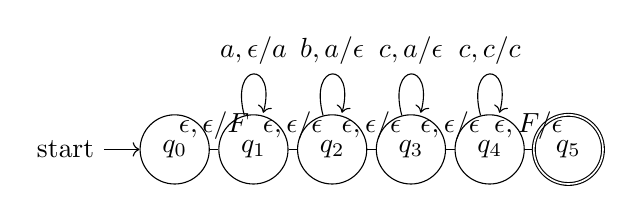
\begin{tikzpicture}
    \node[state, initial] (q0) {$q_0$};
    \node[state, right of=q0] (q1) {$q_1$};
    \node[state, right of=q1] (q2) {$q_2$};
    \node[state, right of=q2] (q3) {$q_3$};
    \node[state, right of=q3] (q4) {$q_4$};
    \node[state, accepting, right of=q4] (q5) {$q_5$};
    \draw
    (q0) edge[above] node{$\epsilon,\epsilon/F$} (q1)
    (q1) edge[loop above] node{$a,\epsilon/a$} (q1)
    (q1) edge[above] node{$\epsilon,\epsilon/\epsilon$} (q2)
    (q2) edge[loop above] node{$b,a/\epsilon$} (q2)
    (q2) edge[above] node{$\epsilon,\epsilon/\epsilon$} (q3)
    (q3) edge[loop above] node{$c,a/\epsilon$} (q3)
    (q3) edge[above] node{$\epsilon,\epsilon/\epsilon$} (q4)
    (q4) edge[loop above] node{$c,c/c$} (q4)
    (q4) edge[above] node{$\epsilon,F/\epsilon$} (q5)
    ;
  \end{tikzpicture}
  \end{figure}
 \item Create a CFG and convert that to a PDA
  \begin{align*}
    S &\rightarrow aST | b \\
    T &\rightarrow Tc | c
  \end{align*}
  \begin{figure}[H]
  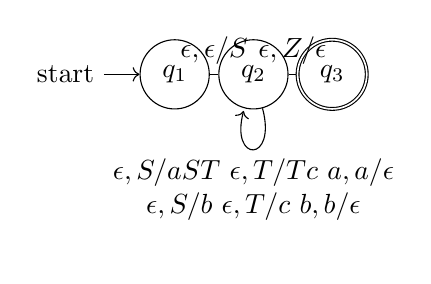
\begin{tikzpicture}
    \node[state, initial] (q1) {$q_1$};
    \node[state, right of=q1] (q2) {$q_2$};
    \node[state, accepting, right of=q2] (q3) {$q_3$};
    \draw
    (q1) edge[above] node{$\epsilon,\epsilon/S$} (q2)
    (q2) edge[loop below] node[align=center]
    {
      $\epsilon,S/aST$  $\epsilon,T/Tc$  $a,a/\epsilon$ \\
      $\epsilon,S/b$  $\epsilon,T/c$  $b,b/\epsilon$ \\
    } (q2)
    (q2) edge[above] node{$\epsilon,Z/\epsilon$} (q3)
    ;
  \end{tikzpicture}
  \end{figure}

\end{itemize}
\newpage
\section*{Problem 3} \textbf{Create a PDA that accepts the language of all
  words with more a's than b's. Don't go through a CFG, use the stack to do the
  work.}

  \begin{figure}[H]
  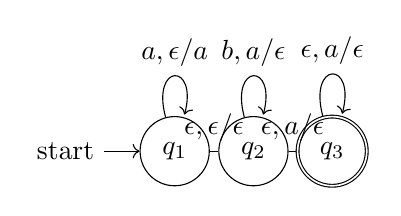
\begin{tikzpicture}
    \node[state, initial] (q1) {$q_1$};
    \node[state, right of=q1] (q2) {$q_2$};
    \node[state, accepting, right of=q2] (q3) {$q_3$};
    \draw
    (q1) edge[loop above] node{$a,\epsilon/a$} (q1)
    (q1) edge[above] node{$\epsilon,\epsilon/\epsilon$} (q2)
    (q2) edge[loop above] node{$b,a/\epsilon$} (q2)
    (q2) edge[above] node{$\epsilon,a/\epsilon$} (q3)
    (q3) edge[loop above] node{$\epsilon,a/\epsilon$} (q3)
    ;
  \end{tikzpicture}
  \end{figure}


\newpage
\section*{Problem 4} \textbf{Prove that CFLs are closed under union.}\\
If we have two CFLs, $L_1$ & $L_2$, they can be represented as CFGs,
$S_1$ & $S_2$.  Then these two CFGs can be used in another CFG as follows

  \begin{align*}
    S &\rightarrow S_1 | S_2 \\
  \end{align*}

This creates a new CFL, so CFLs are closed under union.

\end{document}
